\documentclass[conference]{IEEEtran}

\usepackage{cite}
\usepackage{amsmath,amssymb,amsfonts}
\usepackage{graphicx}
\usepackage{textcomp}
\usepackage{xcolor}
\usepackage{tikz}
\usetikzlibrary{positioning, arrows.meta, shapes.geometric, fit, calc, decorations.pathreplacing}
\usepackage{booktabs}
\usepackage{multirow}
\usepackage{array}
\usepackage{listings}
\usepackage{hyperref}
\usepackage{float}
\usepackage{enumitem}
\usepackage[margin=0.75in]{geometry}

\lstset{
  basicstyle=\ttfamily\scriptsize,
  breaklines=true,
  frame=single,
  columns=fullflexible,
  keepspaces=true
}

\newcolumntype{L}[1]{>{\raggedright\arraybackslash}p{#1}}
\newcolumntype{C}[1]{>{\centering\arraybackslash}p{#1}}

\begin{document}

\title{Dual-FPGA Trading Engine}

\author{
\IEEEauthorblockN{Kushal Agrawal, Eeshana Hari}
\IEEEauthorblockA{Department of Electrical and Computer Engineering, University of Wisconsin--Madison\\
ECE~554 Capstone Design Project, Spring 2026}
}

\maketitle

\begin{abstract}
We present a dual-FPGA deterministic trading engine built on two AMD AUP-ZU3 boards (Zynq UltraScale+ XCZU3EG). Board~A implements an Exchange-Lite with a synthetic market simulator that generates multi-symbol quote streams under four configurable stress regimes. Board~B implements a Trader with a pipelined strategy engine, hardware risk management, and cycle-accurate latency measurement. The boards communicate over a custom full-duplex streaming link using the Pmod+ interface at 50\,MHz, achieving up to 2.78 million frames per second with 8-bit data width. All real-time processing occurs in programmable logic with a deterministic 8-cycle (80\,ns) pipeline latency and zero jitter. A laptop dashboard displays throughput, latency histograms, per-symbol positions, and profit/loss in real time at 20\,Hz via USB-UART telemetry. The architecture is parameterized for symbol count and link width, enabling single-constant scaling from 4 to 256 symbols and 4-bit to 8-bit link without structural changes. Estimated FPGA utilization is under 10\% across all resource types, leaving substantial headroom for extensions.
\end{abstract}

\begin{IEEEkeywords}
FPGA, Zynq UltraScale+, low-latency trading, deterministic processing, hardware measurement, AXI-Lite, fixed-point arithmetic, clock domain crossing, PMOD
\end{IEEEkeywords}

% ===========================================================================
\section{Introduction}
% ===========================================================================

Modern electronic trading systems demand sub-microsecond decision-making with deterministic timing. General-purpose processors running operating systems introduce unpredictable jitter---typically 10--100\,$\mu$s---due to scheduling, cache behavior, and interrupt handling. This jitter makes software-based latency measurement unreliable and software-based trading non-deterministic.

FPGAs offer a fundamentally different execution model: fully pipelined, cycle-deterministic hardware that processes data in a fixed number of clock cycles regardless of workload. This project demonstrates this capability through a closed-loop trading testbed spanning two physically separate FPGA boards.

\subsection{Project Scope}

The system implements a simplified but semantically complete trading loop:
\begin{enumerate}[noitemsep]
  \item Board~A generates synthetic market quotes (bid/ask prices) and sends them to Board~B
  \item Board~B processes quotes through a pipelined strategy and risk engine, then sends orders back
  \item Board~A matches orders against current prices and returns fill or reject responses
  \item Board~B measures round-trip latency in hardware and exposes metrics to a laptop dashboard
\end{enumerate}

Two physically separate boards force real engineering challenges: custom link design, clock domain crossing, and meaningful separation of exchange and trader logic.

\subsection{What This Project Is Not}

This is not a full stock exchange (no deep order book), not algorithmic trading research (the strategy is intentionally simple), and not a networking project (the link is custom PL-to-PL, not Ethernet/TCP). The project is an \textbf{FPGA systems engineering demonstration}: custom interconnect, real-time pipelines, hardware measurement, and a polished demo.

% ===========================================================================
\section{Use-Case Requirements}
% ===========================================================================

Each requirement is traced from a functional need to a technical approach to a quantitative acceptance metric, summarized in Table~\ref{tab:requirements}.

\begin{table*}[t]
\centering
\caption{Design Requirements Matrix}
\label{tab:requirements}
\begin{tabular}{@{}L{2.2cm}L{4.5cm}L{5cm}L{4.5cm}@{}}
\toprule
\textbf{Requirement} & \textbf{Functional Need} & \textbf{Technical Approach} & \textbf{Quantitative Target} \\
\midrule
Processing Speed & Real-time quote processing with no buffering delay & Fully pipelined RTL in PL; no OS in critical path & $\leq$\,10 cycles = 100\,ns; jitter = 0 \\
\addlinespace
Throughput & Handle high quote rates including burst stress & 4/8-bit PMOD link at 50\,MHz; 64-deep FIFOs; backpressure & 1.47--2.78M frames/sec \\
\addlinespace
Connectivity & Full-duplex deterministic inter-board link & Custom streaming bus over Pmod+; mesochronous clocking; valid/ready handshake & Frame loss = 0; BER = 0 \\
\addlinespace
Latency Measurement & Hardware-accurate round-trip measurement & Cycle-counter timestamps echoed in fill messages; 16-bin histogram in PL & Resolution: 10\,ns (1 cycle) \\
\addlinespace
Telemetry & Real-time dashboard for demo & PS reads AXI-Lite registers at 20\,Hz; JSON over USB-UART & 8 panels; 50\,ms refresh \\
\addlinespace
Determinism & Reproducible results given same seed & LFSR PRNG; all logic synchronous; proper CDC & 0-cycle jitter; identical replay \\
\addlinespace
Stress Resilience & Stable under all 4 regimes & FIFO backpressure; error counters & $\geq$\,10\,min/regime; 0 errors \\
\addlinespace
Risk Management & Enforce safety limits in hardware & 3 parallel checks in 1 pipeline stage & 1-cycle check (10\,ns) \\
\bottomrule
\end{tabular}
\end{table*}

% ===========================================================================
\section{System Architecture}
% ===========================================================================

Fig.~\ref{fig:system_overview} shows the complete system topology. Board~A and Board~B communicate over two PMOD ribbon cables (one per direction). Board~B connects to a laptop via USB-UART for telemetry.

\begin{figure}[h]
\centering
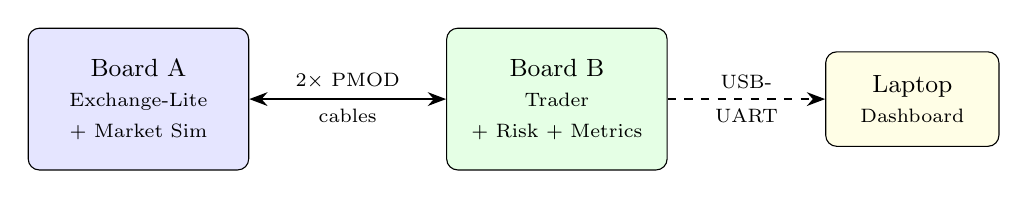
\begin{tikzpicture}[
  board/.style={draw, rounded corners, minimum width=2.8cm, minimum height=1.8cm, align=center, font=\small},
  laptop/.style={draw, rounded corners, minimum width=2.2cm, minimum height=1.2cm, align=center, font=\small},
  link/.style={<->, thick, >=Stealth},
  uartlink/.style={->, thick, >=Stealth, dashed}
]
  \node[board, fill=blue!10] (A) {Board A\\{\scriptsize Exchange-Lite}\\{\scriptsize + Market Sim}};
  \node[board, fill=green!10, right=2.5cm of A] (B) {Board B\\{\scriptsize Trader}\\{\scriptsize + Risk + Metrics}};
  \node[laptop, fill=yellow!10, right=2cm of B] (L) {Laptop\\{\scriptsize Dashboard}};

  \draw[link] (A) -- node[above, font=\scriptsize] {2$\times$ PMOD} node[below, font=\scriptsize] {cables} (B);
  \draw[uartlink] (B) -- node[above, font=\scriptsize] {USB-} node[below, font=\scriptsize] {UART} (L);
\end{tikzpicture}
\caption{System topology: two AUP-ZU3 boards connected via PMOD, laptop for telemetry display.}
\label{fig:system_overview}
\end{figure}

\subsection{Board Roles}

\begin{itemize}[noitemsep]
  \item \textbf{Board~A (Exchange-Lite + Market Simulator):} Generates synthetic quote streams for multiple symbols using an LFSR-driven random walk. Accepts incoming orders and matches them against current bid/ask prices, returning fill or reject responses. Supports four stress regimes (calm, volatile, burst, adversarial) switchable in real time.
  \item \textbf{Board~B (Trader):} Consumes quotes, computes features (EMA, spread), generates trading signals via a mean-reversion strategy, enforces position/rate/loss risk limits, and sends orders. Processes returned fills to update positions, cash, and a 16-bin latency histogram---all in PL.
  \item \textbf{Laptop (Dashboard):} Displays 8 real-time panels: throughput gauges, latency histogram, per-symbol positions, PnL chart, regime indicator, risk reject count, link health, and scalar latency stats.
\end{itemize}

\subsection{Data Lifecycle}

A single trading cycle proceeds as follows:
\begin{enumerate}[noitemsep]
  \item \texttt{market\_sim} on Board~A generates a QUOTE (128-bit frame) with bid/ask prices
  \item Frame serialized over PmodA cable to Board~B at 50\,MHz data rate
  \item Board~B pipeline: demux $\rightarrow$ quote\_book $\rightarrow$ feature\_compute $\rightarrow$ strategy $\rightarrow$ risk $\rightarrow$ order\_manager (8 cycles)
  \item ORDER frame serialized over PmodB cable back to Board~A
  \item \texttt{exchange\_lite} on Board~A matches order: FILL if price favorable, REJECT otherwise
  \item FILL frame sent back to Board~B over PmodA cable
  \item Board~B: position/cash update + latency measurement (cycle\_counter $-$ echoed timestamp)
\end{enumerate}

% ===========================================================================
\section{Demo Approach}
% ===========================================================================

\subsection{Dashboard Panels}

The laptop dashboard displays 8 real-time panels:
\begin{enumerate}[noitemsep]
  \item \textbf{Throughput gauges:} quotes/sec, orders/sec, fills/sec
  \item \textbf{Latency histogram:} 16-bin bar chart with p50/p99/max annotations
  \item \textbf{Position bars:} per-symbol position (green = long, red = short)
  \item \textbf{PnL line chart:} running profit/loss over time
  \item \textbf{Regime indicator:} current stress mode label + color
  \item \textbf{Risk reject counter:} jumps visibly when limits are hit
  \item \textbf{Link health:} error count (should remain 0 throughout demo)
  \item \textbf{Scalar stats:} p50, p99, max latency in nanoseconds
\end{enumerate}

\subsection{Scripted Demo Flow}

\begin{table}[h]
\centering
\caption{Demo Script}
\label{tab:demo}
\begin{tabular}{@{}cL{2.5cm}L{3.5cm}@{}}
\toprule
\textbf{Step} & \textbf{Action} & \textbf{Audience Sees} \\
\midrule
1 & Power on, PYNQ boots & LEDs on, dashboard connects \\
2 & Config Board~A (CALM) & Quotes flowing \\
3 & Enable trading on B & Orders + fills, PnL moves \\
4 & Switch to VOLATILE & Spread widens, PnL swings \\
5 & Switch to BURST & Rate spikes to $>$1M/sec \\
6 & Switch to ADVERSARIAL & Risk rejects spike \\
7 & Return to CALM & System stabilizes \\
8 & Highlight link errors = 0 & Proves zero loss \\
\bottomrule
\end{tabular}
\end{table}

% ===========================================================================
\section{Hardware Platform}
% ===========================================================================

Both boards are AMD AUP-ZU3 featuring a Zynq UltraScale+ XCZU3EG-2SFVC784E with an ARM Cortex-A53 quad-core PS and UltraScale+ PL. Table~\ref{tab:resources} summarizes available and estimated resources.

\begin{table}[h]
\centering
\caption{FPGA Resource Budget (per board)}
\label{tab:resources}
\begin{tabular}{@{}lccc@{}}
\toprule
\textbf{Resource} & \textbf{Available} & \textbf{Est. Used} & \textbf{Util.} \\
\midrule
CLB LUTs       & 70,560  & $\sim$5,000 & $\sim$7\% \\
CLB Flip-Flops & 141,120 & $\sim$4,000 & $\sim$3\% \\
Block RAM (18Kb)& 432    & $\sim$8     & $\sim$2\% \\
DSP48E2 Slices & 360     & $\sim$5     & $\sim$1\% \\
UltraRAM       & 7.6\,Mb & 0           & 0\% \\
\bottomrule
\end{tabular}
\end{table}

\subsection{Clock Architecture}

The design uses PS FCLK0 = 100\,MHz as the single core clock for all PL logic, which is the standard PYNQ approach. This eliminates clock domain crossings between AXI-Lite and the data-plane pipeline. The only CDC boundary is at the link RX, where incoming PMOD data (from the other board's independent oscillator) is synchronized via 2-FF synchronizers.

\subsection{Number Representation}

All prices and monetary values use fixed-point representation to avoid floating-point hardware and maintain determinism. Table~\ref{tab:numfmt} summarizes the formats.

\begin{table}[h]
\centering
\caption{Number Formats}
\label{tab:numfmt}
\begin{tabular}{@{}llll@{}}
\toprule
\textbf{Type} & \textbf{Width} & \textbf{Format} & \textbf{Range} \\
\midrule
Price           & 32 bits & Unsigned Q16.16 & 0 -- 65535.9999 \\
PnL / Signed    & 32 bits & Signed Q16.16   & $\pm$32767.9999 \\
Cash Accum.     & 48 bits & Signed Q32.16   & $\pm$2 billion \\
Quantity        & 16 bits & Unsigned int    & 0 -- 65535 \\
Symbol ID       & 8 bits  & Unsigned int    & 0 -- 255 \\
Order ID        & 16 bits & Unsigned int    & 0 -- 65535 \\
Timestamp       & 16 bits & Unsigned int    & 0 -- 65535 \\
\bottomrule
\end{tabular}
\end{table}

Fixed-point arithmetic rules: addition/subtraction is direct (same format). Price $\times$ quantity uses one DSP48E2: \texttt{result\_48 = price\_32 * qty\_16} yielding Q32.16 for cash accumulation. EMA uses two DSP48E2 slices: \texttt{ema\_new = (alpha * sample + (65536 - alpha) * ema\_old) >> 16}.

\subsection{Power}

Each board is powered via USB-C PD (9\,V at 3\,A). A TPS25730 PD controller negotiates the supply voltage. Under our low utilization ($<$10\%), thermal load is well within the passive heatsink's capacity.

% ===========================================================================
\section{Board-to-Board Link Layer}
% ===========================================================================

\subsection{Physical Interface}

The AUP-ZU3 provides a Pmod+ connector with 22 signal pins: PmodA (JA[0:7]), PmodB (JB[0:7]), and Pmod+ extras (JAB[0:5]), all at LVCMOS33. The link uses two standard 12-pin PMOD ribbon cables in 4-bit mode, with an optional upgrade to 8-bit mode using 4 additional jumper wires on the JAB pins.

Table~\ref{tab:pin_4bit} shows the 4-bit pin assignment. Table~\ref{tab:pin_8bit} shows the 8-bit upgrade.

\begin{table}[h]
\centering
\caption{Pin Assignment: 4-bit Mode (default)}
\label{tab:pin_4bit}
\begin{tabular}{@{}llll@{}}
\toprule
\textbf{Pin} & \textbf{Ball} & \textbf{Signal} & \textbf{A$\rightarrow$B / B$\rightarrow$A} \\
\midrule
\multicolumn{4}{@{}l}{\textit{PmodA cable (A$\rightarrow$B direction):}} \\
JA[0] & J12 & data[0] & A out, B in \\
JA[1] & H12 & data[1] & A out, B in \\
JA[2] & H11 & data[2] & A out, B in \\
JA[3] & G10 & data[3] & A out, B in \\
JA[4] & K13 & tx\_valid & A out, B in \\
JA[5] & K12 & rx\_ready & B out, A in \\
JA[6:7] & J11, J10 & spare & -- \\
\addlinespace
\multicolumn{4}{@{}l}{\textit{PmodB cable (B$\rightarrow$A direction):}} \\
JB[0] & E12 & data[0] & B out, A in \\
JB[1] & D11 & data[1] & B out, A in \\
JB[2] & B11 & data[2] & B out, A in \\
JB[3] & A10 & data[3] & B out, A in \\
JB[4] & C11 & tx\_valid & B out, A in \\
JB[5] & B10 & rx\_ready & A out, B in \\
JB[6:7] & A12, A11 & spare & -- \\
\bottomrule
\end{tabular}
\end{table}

\begin{table}[h]
\centering
\caption{Pin Assignment: 8-bit Mode (upgrade via JAB jumper wires)}
\label{tab:pin_8bit}
\begin{tabular}{@{}llll@{}}
\toprule
\textbf{Pin} & \textbf{Ball} & \textbf{Signal} & \textbf{Dir} \\
\midrule
JA[0:7] & J12..J10 & A$\rightarrow$B data[7:0] & A out \\
JB[0:7] & E12..A11 & B$\rightarrow$A data[7:0] & B out \\
JAB[0] & F12 & A$\rightarrow$B valid & A out \\
JAB[1] & G11 & B$\rightarrow$A valid & B out \\
JAB[2] & E10 & A$\rightarrow$B ready & B out \\
JAB[3] & * & B$\rightarrow$A ready & A out \\
JAB[4:5] & F10, F11 & spare & -- \\
\bottomrule
\multicolumn{4}{@{}l}{\scriptsize * JAB[3] ball to be confirmed from official board XDC.} \\
\end{tabular}
\end{table}

\subsection{Clocking Strategy}

Both boards use independent 100\,MHz clocks (PS FCLK0). Data is output at a 50\,MHz effective rate via a clock-enable toggle, holding each output value for 20\,ns. This respects the PMOD signal speed limit of approximately 50\,MHz documented in the AUP-ZU3 reference manual. No forwarded clock is required; the receiver synchronizes the incoming \texttt{valid} signal through a 2-FF synchronizer and uses it to detect frame boundaries.

\subsection{Frame Protocol}

All messages are 128-bit fixed-size frames. Serialization transmits MSB-first at the configured data width:

\begin{itemize}[noitemsep]
  \item \textbf{4-bit mode:} 32 beats $\times$ 20\,ns = 640\,ns/frame + 40\,ns gap $\rightarrow$ \textbf{1.47M\,fps}
  \item \textbf{8-bit mode:} 16 beats $\times$ 20\,ns = 320\,ns/frame + 40\,ns gap $\rightarrow$ \textbf{2.78M\,fps}
\end{itemize}

The \texttt{valid} signal is asserted for the duration of the frame and deasserted for at least 2 data beats between frames. The \texttt{ready} signal implements backpressure: if the receiver's FIFO approaches capacity, it deasserts \texttt{ready}, and the transmitter pauses after completing the current frame.

% ===========================================================================
\section{Message Format}
% ===========================================================================

Three message types share a universal 128-bit frame. The 4-bit \texttt{msg\_type} field in bits [127:124] distinguishes them. All prices use unsigned Q16.16 fixed-point representation.

\subsection{QUOTE (Board~A $\rightarrow$ Board~B)}

\begin{lstlisting}
[127:124]  msg_type = 4'h1
[123:116]  symbol_id (8 bits)
[115:114]  regime (2 bits)
[113:112]  reserved
[111:80]   bid_price (Q16.16)
[79:48]    ask_price (Q16.16)
[47:32]    bid_size (16-bit qty)
[31:16]    ask_size (16-bit qty)
[15:0]     seq_num (monotonic)
\end{lstlisting}

\subsection{ORDER (Board~B $\rightarrow$ Board~A)}

\begin{lstlisting}
[127:124]  msg_type = 4'h2
[123:116]  symbol_id (8 bits)
[115]      side (0=BUY, 1=SELL)
[114:112]  reserved
[111:80]   limit_price (Q16.16)
[79:64]    quantity (16-bit)
[63:48]    order_id (wrapping counter)
[47:32]    timestamp (cycle_counter[15:0])
[31:0]     reserved
\end{lstlisting}

\subsection{FILL (Board~A $\rightarrow$ Board~B)}

\begin{lstlisting}
[127:124]  msg_type = 4'h3
[123:116]  symbol_id (8 bits)
[115]      side (echoed)
[114:112]  status (000=FILLED, 001=REJECTED)
[111:80]   fill_price (Q16.16)
[79:64]    fill_qty (16-bit)
[63:48]    order_id (echoed)
[47:32]    ts_echo (echoed timestamp)
[31:0]     reserved
\end{lstlisting}

The \texttt{timestamp}/\texttt{ts\_echo} mechanism enables round-trip latency measurement entirely within Board~B's clock domain, avoiding cross-board clock synchronization.

% ===========================================================================
\section{Board~A: Exchange-Lite + Market Simulator}
% ===========================================================================

\begin{figure}[h]
\centering
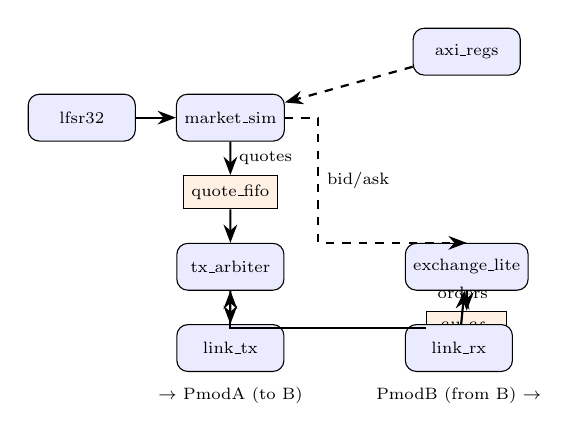
\begin{tikzpicture}[
  mod/.style={draw, rounded corners, minimum width=1.6cm, minimum height=0.7cm, align=center, font=\scriptsize, fill=blue!8},
  fifo/.style={draw, minimum width=1.2cm, minimum height=0.5cm, align=center, font=\scriptsize, fill=orange!10},
  port/.style={font=\scriptsize},
  arr/.style={->, >=Stealth, thick},
  scale=0.85, transform shape
]
  \node[mod] (lfsr) {lfsr32};
  \node[mod, right=0.6 of lfsr] (msim) {market\_sim};
  \node[fifo, below=0.5 of msim] (qfifo) {quote\_fifo};
  \node[mod, below=0.5 of qfifo] (arb) {tx\_arbiter};
  \node[mod, below=0.5 of arb] (ltx) {link\_tx};
  \node[mod, right=1.8 of arb] (exch) {exchange\_lite};
  \node[fifo, below=0.3 of exch] (ffifo) {fill\_fifo};
  \node[mod, right=1.8 of ltx] (lrx) {link\_rx};
  \node[mod, above=2.5 of exch] (regs) {axi\_regs};

  \draw[arr] (lfsr) -- (msim);
  \draw[arr] (msim) -- node[right, font=\scriptsize]{quotes} (qfifo);
  \draw[arr] (qfifo) -- (arb);
  \draw[arr] (arb) -- (ltx);
  \draw[arr] (lrx) -- node[above, font=\scriptsize]{orders} (exch);
  \draw[arr] (exch) -- (ffifo);
  \draw[arr] (ffifo) -| (arb);
  \draw[arr, dashed] (msim.east) -- ++(0.5,0) |- node[near start, right, font=\scriptsize]{bid/ask} (exch.north);
  \draw[arr, dashed] (regs) -- (msim);

  \node[port, below=0.1 of ltx] {$\rightarrow$ PmodA (to B)};
  \node[port, below=0.1 of lrx] {PmodB (from B) $\rightarrow$};
\end{tikzpicture}
\caption{Board~A data-plane architecture. Fills have strict priority over quotes in the TX arbiter.}
\label{fig:board_a}
\end{figure}

\subsection{Market Simulator}

The market simulator maintains per-symbol state (mid-price, spread) and evolves prices using a 32-bit Galois LFSR with polynomial $x^{32}+x^{22}+x^{2}+x+1$. The price update per quote:

\begin{equation}
\text{mid}[s] \mathrel{+}= (\text{lfsr}[4{:}0] - 16) \times \text{step\_size}[\text{regime}]
\end{equation}

Bid and ask prices are derived as $\text{mid} \pm \text{spread}/2$. Four regimes control step size, base spread, and quote interval, as shown in Table~\ref{tab:regimes}.

\begin{table}[h]
\centering
\caption{Market Regime Parameters}
\label{tab:regimes}
\begin{tabular}{@{}lccl@{}}
\toprule
\textbf{Regime} & \textbf{Step Size} & \textbf{Spread} & \textbf{Rate} \\
\midrule
Calm       & $\sim$0.004 & $\sim$\$0.125 & $\sim$100K\,qps \\
Volatile   & $\sim$0.063 & $\sim$\$0.50  & $\sim$200K\,qps \\
Burst      & $\sim$0.004 & $\sim$\$0.125 & $\sim$1.4M\,qps \\
Adversarial& $\sim$0.250 & $\sim$\$1.00  & $\sim$1M\,qps \\
\bottomrule
\end{tabular}
\end{table}

\subsection{Exchange-Lite Matching}

The matcher implements a simple rule: a BUY order fills if \texttt{limit\_price} $\geq$ \texttt{ask\_price}; a SELL order fills if \texttt{limit\_price} $\leq$ \texttt{bid\_price}. Otherwise the order is rejected. No resting orders or order book depth---intentionally simplified to keep scope manageable while maintaining a truthful ``exchange'' story.

% ===========================================================================
\section{Board~B: Trader}
% ===========================================================================

\begin{figure}[h]
\centering
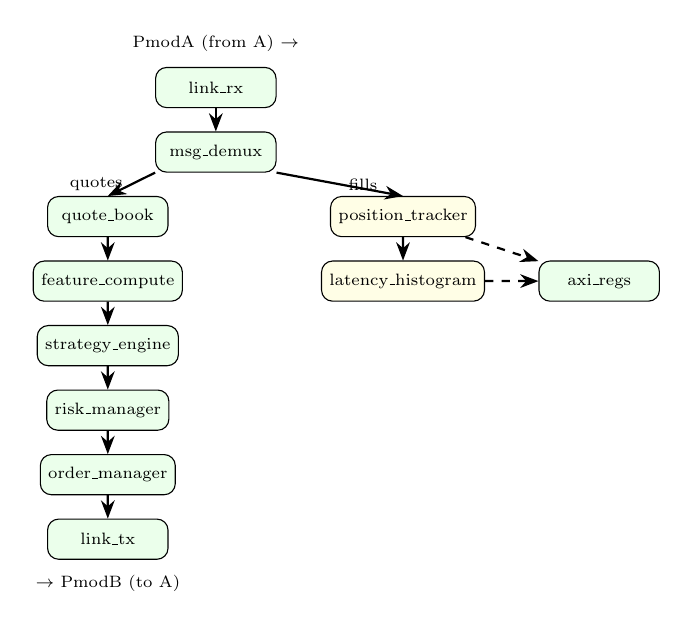
\begin{tikzpicture}[
  mod/.style={draw, rounded corners, minimum width=1.8cm, minimum height=0.6cm, align=center, font=\scriptsize, fill=green!8},
  port/.style={font=\scriptsize},
  arr/.style={->, >=Stealth, thick},
  scale=0.85, transform shape
]
  \node[mod] (lrx) {link\_rx};
  \node[mod, below=0.35 of lrx] (demux) {msg\_demux};
  \node[mod, below left=0.35 and -0.2 of demux] (qb) {quote\_book};
  \node[mod, below=0.35 of qb] (fc) {feature\_compute};
  \node[mod, below=0.35 of fc] (se) {strategy\_engine};
  \node[mod, below=0.35 of se] (rm) {risk\_manager};
  \node[mod, below=0.35 of rm] (om) {order\_manager};
  \node[mod, below=0.35 of om] (ltx) {link\_tx};

  \node[mod, below right=0.35 and 0.8 of demux, fill=yellow!10] (pt) {position\_tracker};
  \node[mod, below=0.35 of pt, fill=yellow!10] (lh) {latency\_histogram};
  \node[mod, right=0.8 of lh] (regs) {axi\_regs};

  \draw[arr] (lrx) -- (demux);
  \draw[arr] (demux.south west) -- node[left, font=\scriptsize]{quotes} (qb.north);
  \draw[arr] (demux.south east) -- node[right, font=\scriptsize]{fills} (pt.north);
  \draw[arr] (qb) -- (fc);
  \draw[arr] (fc) -- (se);
  \draw[arr] (se) -- (rm);
  \draw[arr] (rm) -- (om);
  \draw[arr] (om) -- (ltx);
  \draw[arr] (pt) -- (lh);
  \draw[arr, dashed] (lh) -- (regs);
  \draw[arr, dashed] (pt) -- (regs);

  \node[port, above=0.1 of lrx] {PmodA (from A) $\rightarrow$};
  \node[port, below=0.1 of ltx] {$\rightarrow$ PmodB (to A)};
\end{tikzpicture}
\caption{Board~B architecture. Left path: quote-to-order pipeline (8 cycles). Right path: fill processing (position + latency).}
\label{fig:board_b}
\end{figure}

\subsection{Pipeline Stages}

Table~\ref{tab:pipeline} details the 8-stage pipeline from quote arrival to order dispatch.

\begin{table}[h]
\centering
\caption{Board~B Pipeline Breakdown}
\label{tab:pipeline}
\begin{tabular}{@{}clcl@{}}
\toprule
\textbf{Stage} & \textbf{Module} & \textbf{Cycles} & \textbf{Operation} \\
\midrule
1 & msg\_demux & 1 & Route by msg\_type \\
2 & quote\_book & 1 & Update bid/ask registers \\
3 & feature\_compute & 1 & mid, spread \\
4--5 & feature\_compute & 2 & EMA (DSP48 multiply) \\
6 & strategy\_engine & 1 & Deviation vs threshold \\
7 & risk\_manager & 1 & 3 parallel limit checks \\
8 & order\_manager & 1 & Build ORDER frame \\
\midrule
& \textbf{Total} & \textbf{8} & \textbf{80\,ns at 100\,MHz} \\
\bottomrule
\end{tabular}
\end{table}

\subsection{Strategy: Mean Reversion}

The strategy computes an exponential moving average (EMA) of the mid-price using two DSP48E2 slices for fixed-point multiplication:
\begin{equation}
\text{ema}_{\text{new}} = \frac{\alpha \cdot \text{mid} + (65536 - \alpha) \cdot \text{ema}_{\text{old}}}{65536}
\end{equation}
where $\alpha$ is a Q0.16 parameter (default 6554 $\approx$ 0.1). A trade signal is generated when $|\text{mid} - \text{ema}| > \text{threshold}$: if mid $>$ ema + threshold, SELL at bid\_price (aggressive); if mid $<$ ema $-$ threshold, BUY at ask\_price (aggressive). Quote generation is round-robin across symbols: each timer tick produces one quote for the next symbol in sequence.

\subsection{Risk Management}

Three independent checks execute in parallel in a single cycle:
\begin{enumerate}[noitemsep]
  \item \textbf{Position limit:} $|\text{position}[s] + \text{signed\_qty}| \leq \text{max\_position}$
  \item \textbf{Order rate:} orders in sliding window $<$ max\_rate
  \item \textbf{Loss halt:} total PnL $> -$max\_loss
\end{enumerate}
All three must pass for an order to be approved. Any failure suppresses the order and increments a reject counter readable via AXI-Lite.

\subsection{Latency Measurement}

Board~B maintains a free-running 16-bit cycle counter. When an ORDER is sent, \texttt{cycle\_counter[15:0]} is embedded as the timestamp. When the FILL returns, the echoed timestamp is subtracted:
\begin{equation}
\text{latency} = \text{cycle\_counter}_{\text{now}} - \text{ts\_echo}
\end{equation}
This 16-bit wrapping subtraction is valid as long as the round-trip is less than $2^{16}$ cycles (655\,$\mu$s at 100\,MHz). Results are accumulated into a 16-bin histogram with 32-cycle (320\,ns) bin width, plus min, max, sum, and count registers. The laptop computes p50 and p99 from the histogram's cumulative distribution.

% ===========================================================================
\section{Software Architecture}
% ===========================================================================

\subsection{PS Software (PYNQ)}

The ARM Cortex-A53 runs PYNQ Linux. No soft-core processor (MicroBlaze) is instantiated in PL. The PS handles two tasks:

\begin{itemize}[noitemsep]
  \item \textbf{Board~A:} \texttt{config\_exchange.py} loads the overlay, writes regime parameters, initial prices, LFSR seed, and start bit via \texttt{pynq.MMIO}.
  \item \textbf{Board~B:} \texttt{telemetry\_server.py} polls AXI-Lite registers at 20\,Hz and prints JSON lines to UART.
\end{itemize}

\subsection{UART Telemetry Protocol}

Board~B PS sends one JSON line every 50\,ms to the FTDI UART (COM port):

\begin{lstlisting}
{"qps":125000,"ops":5000,"fps":4950,"rej":42,
 "pos":[10,-5,0,0],"cash_lo":1234,"cash_hi":0,
 "hist":[100,500,300,50,10,0,0,0,0,0,0,0,0,0,0,0],
 "lat_min":28,"lat_max":487,"lat_cnt":4950,
 "link_err":0}
\end{lstlisting}

At 115200 baud ($\sim$11.5\,KB/s capacity), a $\sim$200-byte JSON line every 50\,ms requires only $\sim$4\,KB/s---well within capacity. Baud rate is upgradeable to 921600 if needed.

Rate computation on the laptop: counters are monotonic, so \texttt{rate = (counter\_now - counter\_prev) / delta\_time}. Percentiles: walk histogram bins cumulatively; p50 = bin where cumulative $\geq$ 50\% of total.

\subsection{Laptop Dashboard}

A Python Plotly Dash web application (\texttt{localhost:8050}) reads JSON lines from USB-UART via \texttt{pyserial} and displays 8 real-time panels: throughput gauges, latency histogram with p50/p99 annotations, per-symbol position bars, running PnL chart, regime indicator, risk reject counter, link health status, and scalar latency statistics.

% ===========================================================================
\section{Submodule Catalog}
% ===========================================================================

The design comprises 22 RTL modules and 4 testbenches, listed in Table~\ref{tab:modules}. All data-plane modules use a valid/ready handshake: transfer occurs when both \texttt{valid} and \texttt{ready} are asserted on the same rising clock edge.

\begin{table}[h]
\centering
\caption{Complete Module List}
\label{tab:modules}
\begin{tabular}{@{}clll@{}}
\toprule
\textbf{\#} & \textbf{Module} & \textbf{Board} & \textbf{Type} \\
\midrule
1 & hft\_pkg.sv & Shared & Package \\
2 & lfsr32.sv & Shared & Logic \\
3 & debounce.sv & Shared & Logic \\
4 & link\_tx.sv & Shared & Serializer \\
5 & link\_rx.sv & Shared & Deserializer \\
\addlinespace
6 & market\_sim.sv & A & DSP+Logic \\
7 & exchange\_lite.sv & A & Logic \\
8 & tx\_arbiter.sv & A & Logic \\
9 & board\_a\_axi\_regs.sv & A & AXI-Lite \\
10 & board\_a\_ctrl.sv & A & Logic \\
11 & board\_a\_top.sv & A & Structural \\
\addlinespace
12 & msg\_demux.sv & B & Logic \\
13 & quote\_book.sv & B & Registers \\
14 & feature\_compute.sv & B & DSP+Logic \\
15 & strategy\_engine.sv & B & Logic \\
16 & risk\_manager.sv & B & Logic \\
17 & order\_manager.sv & B & Logic \\
18 & position\_tracker.sv & B & DSP+Logic \\
19 & latency\_histogram.sv & B & Logic \\
20 & board\_b\_axi\_regs.sv & B & AXI-Lite \\
21 & board\_b\_ctrl.sv & B & Logic \\
22 & board\_b\_top.sv & B & Structural \\
\bottomrule
\end{tabular}
\end{table}

\subsection{Module Interface Definitions}

Every data-plane module uses a valid/ready handshake: the producer drives \texttt{out\_frame[127:0]} and \texttt{out\_valid}; the consumer drives \texttt{out\_ready}. Transfer occurs when both are high on the same rising edge. Key module interfaces are specified below.

\textbf{link\_tx:} Inputs: \texttt{clk}, \texttt{rst}, \texttt{frame\_in[127:0]}, \texttt{frame\_in\_valid}, \texttt{remote\_ready}. Outputs: \texttt{frame\_in\_ready}, \texttt{pmod\_data[3:0]}, \texttt{pmod\_valid}. Internal: \texttt{tick} (50\,MHz enable), \texttt{nibble\_counter[4:0]}, \texttt{frame\_shift[127:0]}.

\textbf{link\_rx:} Inputs: \texttt{clk}, \texttt{rst}, \texttt{pmod\_data[3:0]}, \texttt{pmod\_valid}. Outputs: \texttt{frame\_out[127:0]}, \texttt{frame\_out\_valid}, \texttt{pmod\_ready}, \texttt{error\_count[31:0]}. Internal: \texttt{valid\_sync[1:0]} (2-FF), \texttt{data\_sync[3:0]} (2-FF per bit), \texttt{nibble\_counter[4:0]}, \texttt{frame\_assemble[127:0]}.

\textbf{market\_sim:} Inputs: \texttt{clk}, \texttt{rst}, \texttt{start}, \texttt{regime[1:0]}, \texttt{quote\_interval[31:0]}, \texttt{num\_symbols[2:0]}, per-symbol init arrays (\texttt{sym\_init\_mid[0:3]}, \texttt{sym\_init\_spread[0:3]}), \texttt{lfsr\_seed[31:0]}. Outputs: \texttt{quote\_frame[127:0]}, \texttt{quote\_valid}, \texttt{bid\_price[0:3]}, \texttt{ask\_price[0:3]}, \texttt{quotes\_sent[31:0]}.

\textbf{exchange\_lite:} Inputs: \texttt{clk}, \texttt{rst}, \texttt{order\_frame[127:0]}, \texttt{order\_valid}, \texttt{bid\_price[0:3]}, \texttt{ask\_price[0:3]}. Outputs: \texttt{fill\_frame[127:0]}, \texttt{fill\_valid}, \texttt{order\_ready}, counters (\texttt{orders\_received}, \texttt{fills\_sent}, \texttt{rejects\_sent}).

\textbf{feature\_compute:} Inputs: \texttt{clk}, \texttt{rst}, \texttt{bid\_price[31:0]}, \texttt{ask\_price[31:0]}, \texttt{symbol\_id[7:0]}, \texttt{quote\_valid}, \texttt{ema\_alpha[15:0]}. Outputs: \texttt{mid\_price[31:0]}, \texttt{spread[31:0]}, \texttt{ema[31:0]}, \texttt{deviation[31:0]} (signed), \texttt{feature\_valid}, \texttt{symbol\_id\_out[7:0]}.

\textbf{strategy\_engine:} Inputs: \texttt{clk}, \texttt{rst}, \texttt{deviation[31:0]}, \texttt{bid\_price[31:0]}, \texttt{ask\_price[31:0]}, \texttt{symbol\_id[7:0]}, \texttt{feature\_valid}, \texttt{threshold[31:0]}, \texttt{base\_qty[15:0]}. Outputs: \texttt{order\_side}, \texttt{order\_price[31:0]}, \texttt{order\_qty[15:0]}, \texttt{order\_symbol[7:0]}, \texttt{signal\_valid}.

\textbf{risk\_manager:} Inputs: \texttt{signal\_valid}, \texttt{order\_side/price/qty/symbol}, \texttt{position[0:3]}, \texttt{total\_pnl[31:0]}, configurable limits (\texttt{max\_position}, \texttt{max\_order\_rate}, \texttt{max\_loss}), \texttt{trading\_enable}. Outputs: \texttt{approved\_valid}, pass-throughs, \texttt{risk\_rejects[31:0]}, \texttt{risk\_halt}.

\textbf{latency\_histogram:} Inputs: \texttt{clk}, \texttt{rst}, \texttt{fill\_valid}, \texttt{ts\_echo[15:0]}, \texttt{cycle\_counter[15:0]}. Outputs (AXI-Lite readable): \texttt{hist\_bins[0:15]} (16$\times$32-bit), \texttt{lat\_min[15:0]}, \texttt{lat\_max[15:0]}, \texttt{lat\_sum[47:0]}, \texttt{lat\_count[31:0]}.

% ===========================================================================
\section{Control Logic and I/O}
% ===========================================================================

The PS is used only for slow-path configuration and telemetry. Real-time control inputs come from physical switches and buttons, processed by a \texttt{board\_x\_ctrl} module with debounce logic (20\,ms filter).

\subsection{Board~A I/O Assignment}

\begin{itemize}[noitemsep]
  \item \textbf{SW[1:0]} (AB1, AF1): Regime select (00=calm, 01=volatile, 10=burst, 11=adversarial)
  \item \textbf{SW[2]} (AE3): Override source (0=PS register, 1=switches)
  \item \textbf{SW[3:7]} (AC2, AC1, AD6, AD1, AD2): Reserved
  \item \textbf{BTN[0/1/2]} (AB6, AB7, AB2): Start / Stop / Reset; \textbf{BTN[3]} (AC6): Reserved
  \item \textbf{LED[3:0]} (AF5, AE7, AH2, AE5): Regime indicator (binary + blink when running)
  \item \textbf{LED[7:4]} (AH1, AE4, AG1, AF2): Link activity (flash on TX/RX)
  \item \textbf{RGB0} (AD7/AD9/AE9): Regime color (green=calm, yellow=volatile, red=burst, purple=adversarial)
  \item \textbf{RGB1} (AG9/AE8/AF8): Link health (green=OK, red=errors)
\end{itemize}

\subsection{Board~B I/O Assignment}

\begin{itemize}[noitemsep]
  \item \textbf{SW[0]} (AB1): Trading enable (0=observe, 1=trade)
  \item \textbf{SW[1:7]}: Reserved
  \item \textbf{BTN[0/1/2]} (AB6, AB7, AB2): Start / Stop / Reset; \textbf{BTN[3]} (AC6): Reserved
  \item \textbf{LED[3:0]} (AF5, AE7, AH2, AE5): Order activity (flash per order)
  \item \textbf{LED[7:4]} (AH1, AE4, AG1, AF2): Fill activity (flash per fill)
  \item \textbf{RGB0} (AD7/AD9/AE9): PnL (green=profit, red=loss, off=flat)
  \item \textbf{RGB1} (AG9/AE8/AF8): Risk status (green=OK, yellow=$>$80\%, red=halted)
\end{itemize}

All GPIO pins use LVCMOS12 (switches, LEDs, RGBs) or LVCMOS33 (buttons, PMODs), matching the AUP-ZU3 I/O bank assignments documented in the reference manual.

\subsection{Debounce and Edge Detection}

All four buttons pass through \texttt{debounce.sv}: a 20-bit shift register clocked at 100\,MHz. The output changes only when all 20 samples agree ($\sim$200\,$\mu$s debounce window). After debounce, a 1-cycle rising-edge pulse is generated. The \texttt{board\_x\_ctrl} module ORs this pulse with the corresponding AXI-Lite register write, so either hardware button or PS software can trigger the same action.

\subsection{Board~A Operational States}

Board~A operates in four states: RESET (clear counters/FIFOs/LFSR, load initial prices), IDLE (waiting for start; PS writes config), RUNNING (\texttt{market\_sim} generating quotes, \texttt{exchange\_lite} accepting orders, regime selectable at any time), and STOPPED (quotes paused, exchange drains pending orders/fills). Transitions: RESET $\rightarrow$ IDLE (reset done), IDLE $\rightarrow$ RUNNING (start), RUNNING $\leftrightarrow$ STOPPED (stop/start), any $\rightarrow$ RESET (reset button).

\subsection{Board~B Operational States}

Board~B operates in four states: IDLE (no quotes received, waiting for link), ARMED (quotes flowing, features computed, orders NOT sent), TRADING (full pipeline active, orders generated and sent), and HALTED (max loss breached, orders suppressed, must reset). Transitions: IDLE $\rightarrow$ ARMED (link\_up), ARMED $\rightarrow$ TRADING (trading\_enable + start), TRADING $\rightarrow$ ARMED (stop/disable), TRADING $\rightarrow$ HALTED (PnL $< -$max\_loss), any $\rightarrow$ IDLE (reset).

% ===========================================================================
\section{Vivado Build Strategy}
% ===========================================================================

\subsection{Block Design Structure}

The Vivado block design (identical structure for both boards) contains: (1)~Zynq UltraScale+ PS IP with FCLK0 = 100\,MHz and M\_AXI\_HPM0\_LPD master, (2)~Processor System Reset, (3)~AXI Interconnect (1 master, 1 slave), and (4)~our custom IP (\texttt{board\_x\_custom\_ip}) containing all RTL modules as an AXI-Lite slave. The custom IP exposes external ports: \texttt{pmoda[7:0]}, \texttt{pmodb[7:0]}, \texttt{sw[7:0]}, \texttt{btn[3:0]}, \texttt{led[7:0]}, \texttt{rgb[11:0]}.

\subsection{IP Packaging}

We use Vivado's ``Create and Package New IP'' wizard to generate an AXI4-Lite slave template with auto-generated handshake logic. We edit the template to add custom register read/write behavior, instantiate all data-plane RTL modules inside the IP wrapper, and expose PMOD/LED/switch/button ports as top-level IP ports.

\subsection{PYNQ Overlay}

The Vivado build produces a \texttt{.bit} (bitstream) and \texttt{.hwh} (hardware handoff) file, both placed on the MicroSD card. PYNQ's \texttt{Overlay()} class loads them:

\begin{lstlisting}[language=Python]
from pynq import Overlay
ol = Overlay('board_a.bit')
\end{lstlisting}

% ===========================================================================
\section{Parameterization}
% ===========================================================================

Two compile-time parameters enable post-bring-up scaling without architectural changes:

\begin{itemize}[noitemsep]
  \item \textbf{\texttt{NUM\_SYMBOLS}} (default 4): Controls the number of independently traded instruments. Per-symbol arrays are sized by this parameter using \texttt{generate} blocks. The 8-bit \texttt{symbol\_id} field supports up to 256 symbols. Resource cost is $\sim$208 FFs per symbol ($<$0.15\% of available FFs).
  \item \textbf{\texttt{LINK\_DATA\_W}} (default 4): Controls PMOD data bus width. Affects only \texttt{link\_tx} and \texttt{link\_rx}, which derive beat counts as \texttt{FRAME\_WIDTH / LINK\_DATA\_W}. Upgrading from 4 to 8 halves frame latency and doubles throughput.
\end{itemize}

Planned progression: 4~symbols / 4-bit link for bring-up (weeks 1--7), then 8~symbols / 8-bit link for demo (weeks 8--10).

% ===========================================================================
\section{Verification and Testing}
% ===========================================================================

\subsection{Unit Testing}

Every module has a self-checking SystemVerilog testbench. Table~\ref{tab:unit_tests} summarizes the key verification targets.

\begin{table*}[t]
\centering
\caption{Unit Test Matrix}
\label{tab:unit_tests}
\begin{tabular}{@{}lL{4cm}L{4cm}L{4cm}@{}}
\toprule
\textbf{Module} & \textbf{Stimulus} & \textbf{Key Checks} & \textbf{Edge Cases} \\
\midrule
lfsr32 & Seed, clock 100 cycles & Never zero; matches polynomial & seed=0 (prevented), all-ones \\
link\_tx & 5 known frames & Correct nibble sequence MSB-first; valid for 64 clk cycles & Back-to-back; ready deassert mid-idle \\
link\_rx & Known pin pattern & 128-bit match; valid pulses once & Glitch on valid; valid low \\
link loopback & 1000 random frames & All received identical & Max rate; intermittent pauses \\
market\_sim & CALM 100 quotes & Prices in range; spread $>$ 0 & Regime change mid-run; 1 symbol \\
exchange\_lite & BUY at ask & FILL with correct price & Below ask (reject); exact boundary \\
tx\_arbiter & Simultaneous fill+quote & Fill first & Only quotes; only fills \\
msg\_demux & Mixed QUOTE+FILL & Correct routing & Unknown msg\_type (discard) \\
feature\_compute & Known bid/ask & mid exact; EMA converges & Large jump; spread=0; alpha extremes \\
strategy\_engine & Deviation $>$ threshold & Correct BUY/SELL & At threshold exactly; deviation=0 \\
risk\_manager & Position at limit & Rejected + counter & max-1 (approve); rate at max \\
order\_manager & Approved signal & Correct frame; ID increment & Rapid wrap; no signal \\
position\_tracker & BUY then SELL fill & Position/cash correct & Large qty; signed overflow \\
latency\_histogram & Known ts\_echo & Correct bin; min/max updated & latency=0; overflow bin; wrap \\
\bottomrule
\end{tabular}
\end{table*}

\subsection{Integration Testing}

\begin{itemize}[noitemsep]
  \item \textbf{Board~A standalone:} market\_sim + exchange\_lite with synthetic orders (10K quotes)
  \item \textbf{Board~B standalone:} synthetic quote generator replaces link\_rx (5K quotes)
  \item \textbf{Full system:} Board~A + Board~B with behavioral link model (50K quotes, all 4 regimes)
\end{itemize}

\subsection{Hardware Bring-Up}

Nine gated phases ensure incremental verification:

\begin{table}[h]
\centering
\caption{Hardware Bring-Up Phases}
\label{tab:bringup}
\begin{tabular}{@{}clL{3.8cm}@{}}
\toprule
\textbf{Ph.} & \textbf{Goal} & \textbf{Pass Criteria} \\
\midrule
1 & LED blinker       & LED toggles at expected rate \\
2 & AXI-Lite smoke    & Write 0xDEADBEEF, read back \\
3 & Board~A standalone& Counters increment via MMIO \\
4 & Board~B standalone& Orders generated, histogram populated \\
5 & Link smoke test   & tx\_count = rx\_count, 0 errors \\
6 & One-way quotes    & Quote counters match both boards \\
7 & Closed loop       & fill\_count $>$ 0, PnL updating \\
8 & Dashboard         & All 8 panels updating \\
9 & Stress test       & 10\,min/regime, 0 link errors \\
\bottomrule
\end{tabular}
\end{table}

\subsection{Stress Testing Protocol}

\begin{table}[h]
\centering
\caption{Stress Test Protocol}
\label{tab:stress}
\begin{tabular}{@{}lL{1.5cm}L{3.5cm}@{}}
\toprule
\textbf{Regime} & \textbf{Duration} & \textbf{Expected Behavior} \\
\midrule
Calm       & 10 min & $\sim$100K qps, steady PnL \\
Volatile   & 10 min & Same throughput, wider PnL swings \\
Burst      & 10 min & $\sim$1M+ qps, FIFO fill $<$ 75\% \\
Adversarial& 10 min & High rejects, position limits hit \\
Rapid Switch & 10 min & Regime every 30s, no glitches \\
\bottomrule
\end{tabular}
\end{table}

\subsection{Acceptance Criteria}

\begin{table}[h]
\centering
\caption{Acceptance Criteria Matrix}
\label{tab:acceptance}
\begin{tabular}{@{}L{2.2cm}L{2cm}L{2.5cm}@{}}
\toprule
\textbf{Criterion} & \textbf{Target} & \textbf{Verification} \\
\midrule
Closed loop & Full cycle runs & All counters incrementing \\
Determinism & 0-cycle jitter & Single histogram bin \\
Throughput & $\geq$1M qps (burst) & Dashboard gauge \\
Latency & $<$3\,$\mu$s typical & Histogram p99 \\
Reliability & 0 frames lost (10 min) & link\_error = 0 \\
Risk enforce & Position $\leq$ limit & max(abs(pos)) check \\
Telemetry & 8 panels @ $\geq$10 Hz & Visual confirmation \\
Stress & 0 errors all regimes & link\_error after suite \\
\bottomrule
\end{tabular}
\end{table}

% ===========================================================================
\section{Project Management}
% ===========================================================================

\subsection{Schedule}

\begin{table}[h]
\centering
\caption{10-Week Implementation Schedule}
\label{tab:schedule}
\begin{tabular}{@{}cL{3cm}L{3cm}@{}}
\toprule
\textbf{Wk} & \textbf{Kushal (Link + Board~A)} & \textbf{Eeshana (Board~B + Dashboard)} \\
\midrule
1--2 & hft\_pkg, link\_tx/rx, lfsr32 & msg\_demux, quote\_book, feature\_compute \\
3--4 & market\_sim, exchange, arbiter & strategy, risk, order\_mgr \\
5 & Board~A top + testbenches & Board~B top + testbenches \\
6 & Vivado Board~A, Phase 2--3 & Vivado Board~B, Phase 3--4 \\
7 & \multicolumn{2}{c}{Link bring-up (Phase 4--5) --- both together} \\
8 & \multicolumn{2}{c}{Close the loop (Phase 6--7) --- both together} \\
9 & Stress testing (Phase 8--9) & Dashboard + telemetry script \\
10 & \multicolumn{2}{c}{Demo polish + presentation} \\
\bottomrule
\end{tabular}
\end{table}

\subsection{Team Member Responsibilities}

Kushal holds primary responsibility for the link layer, Board~A logic (market simulator, exchange, arbiter), Vivado build infrastructure, and XDC constraints. Secondary responsibilities include assisting with cross-board integration testing and PYNQ overlay packaging.

Eeshana holds primary responsibility for the Board~B trader pipeline (feature computation, strategy, risk, position tracking, latency histogram), the laptop dashboard, and PS telemetry scripts. Secondary responsibilities include assisting with hardware bring-up and demo preparation.

Both team members collaborate on Phase~7--8 (cross-board integration) and share responsibility for testbenches. Phases are gated: each must pass before proceeding to minimize rework.

% ===========================================================================
\section{Risk Analysis}
% ===========================================================================

\begin{table}[h]
\centering
\caption{Risk Assessment and Mitigations}
\label{tab:risks}
\begin{tabular}{@{}L{2.2cm}ccL{3cm}@{}}
\toprule
\textbf{Risk} & \textbf{Prob.} & \textbf{Impact} & \textbf{Mitigation} \\
\midrule
PMOD signal integrity & Low & High & Manual confirms 50\,MHz. Fallback: 25\,MHz. \\
\addlinespace
Mesochronous metastability & Low & High & 2-FF sync. Fallback: forwarded clock via spare pin. \\
\addlinespace
AXI-Lite integration & Med & Med & Vivado auto-gen template; test Phase~2 early. \\
\addlinespace
Fixed-point overflow & Low & Med & 48-bit cash accumulator; saturation logic. \\
\addlinespace
FIFO overflow (BURST) & Low & High & 64-deep FIFOs + backpressure. Monitor fill levels. \\
\addlinespace
PYNQ overlay packaging & Med & Med & Follow PYNQ docs. Test Phase~1--2 early. \\
\addlinespace
Board thermal & Low & Med & $<$10\% utilization; passive heatsink included. \\
\addlinespace
Time pressure & High & High & Phase-gated milestones; cut stretch goals early. \\
\bottomrule
\end{tabular}
\end{table}

% ===========================================================================
\section{Bill of Materials}
% ===========================================================================

\begin{table}[h]
\centering
\caption{Required Hardware}
\label{tab:bom}
\begin{tabular}{@{}llcl@{}}
\toprule
\textbf{Item} & \textbf{Spec} & \textbf{Qty} & \textbf{Purpose} \\
\midrule
AUP-ZU3 board & XCZU3EG & 2 & Compute platforms \\
MicroSD card & 32GB UHS-I & 2 & PYNQ boot image \\
USB-C PD supply & 9V/3A+ & 2 & Board power \\
USB-C data cable & -- & 2 & JTAG + UART \\
PMOD ribbon cable & 12-pin, 2$\times$6 & 2 & Inter-board link \\
Jumper wires & F-F Dupont & 4 & JAB pins (8-bit) \\
\midrule
\multicolumn{4}{@{}l}{\textit{Optional:}} \\
Jumper wires (spare) & F-F Dupont & 20 & Backup for PMOD cables \\
External monitor & HDMI/USB-C & 1 & Demo display \\
\bottomrule
\end{tabular}
\end{table}

% ===========================================================================
\section{Summary}
% ===========================================================================

We present a dual-FPGA deterministic trading engine that implements a complete quote $\rightarrow$ order $\rightarrow$ fill closed loop across two AUP-ZU3 boards. The design achieves sub-100\,ns pipeline latency with zero jitter, cycle-accurate hardware latency measurement via a 16-bin histogram, and up to 2.78 million frames per second over a custom Pmod+ streaming link. All metrics are displayed on a real-time laptop dashboard.

The architecture is parameterized for both symbol count and link width, enabling a smooth progression from 4-symbol/4-bit bring-up to 8-symbol/8-bit demo configuration with single-constant changes. Estimated resource utilization is under 10\% across all FPGA resource types, leaving substantial headroom for future extensions such as neural network strategies or deeper order books.

The 10-week implementation plan is structured around 9 gated hardware bring-up phases, with the critical cross-board integration milestone targeted for week~7--8 and three weeks of buffer before the final demo.

% ===========================================================================
\appendix
% ===========================================================================

\section{XDC Constraints}
\label{app:xdc}

These constraints are identical for Board~A and Board~B (same physical board). Pin direction is controlled by top-level RTL port declarations.

\begin{lstlisting}
## -- PMOD A (LVCMOS33) --
set_property -dict {PACKAGE_PIN J12 IOSTANDARD LVCMOS33} [get_ports {pmoda[0]}]
set_property -dict {PACKAGE_PIN H12 IOSTANDARD LVCMOS33} [get_ports {pmoda[1]}]
set_property -dict {PACKAGE_PIN H11 IOSTANDARD LVCMOS33} [get_ports {pmoda[2]}]
set_property -dict {PACKAGE_PIN G10 IOSTANDARD LVCMOS33} [get_ports {pmoda[3]}]
set_property -dict {PACKAGE_PIN K13 IOSTANDARD LVCMOS33} [get_ports {pmoda[4]}]
set_property -dict {PACKAGE_PIN K12 IOSTANDARD LVCMOS33} [get_ports {pmoda[5]}]
set_property -dict {PACKAGE_PIN J11 IOSTANDARD LVCMOS33} [get_ports {pmoda[6]}]
set_property -dict {PACKAGE_PIN J10 IOSTANDARD LVCMOS33} [get_ports {pmoda[7]}]

## -- PMOD B (LVCMOS33) --
set_property -dict {PACKAGE_PIN E12 IOSTANDARD LVCMOS33} [get_ports {pmodb[0]}]
set_property -dict {PACKAGE_PIN D11 IOSTANDARD LVCMOS33} [get_ports {pmodb[1]}]
set_property -dict {PACKAGE_PIN B11 IOSTANDARD LVCMOS33} [get_ports {pmodb[2]}]
set_property -dict {PACKAGE_PIN A10 IOSTANDARD LVCMOS33} [get_ports {pmodb[3]}]
set_property -dict {PACKAGE_PIN C11 IOSTANDARD LVCMOS33} [get_ports {pmodb[4]}]
set_property -dict {PACKAGE_PIN B10 IOSTANDARD LVCMOS33} [get_ports {pmodb[5]}]
set_property -dict {PACKAGE_PIN A12 IOSTANDARD LVCMOS33} [get_ports {pmodb[6]}]
set_property -dict {PACKAGE_PIN A11 IOSTANDARD LVCMOS33} [get_ports {pmodb[7]}]

## -- Switches (LVCMOS12) --
set_property -dict {PACKAGE_PIN AB1 IOSTANDARD LVCMOS12} [get_ports {sw[0]}]
set_property -dict {PACKAGE_PIN AF1 IOSTANDARD LVCMOS12} [get_ports {sw[1]}]
set_property -dict {PACKAGE_PIN AE3 IOSTANDARD LVCMOS12} [get_ports {sw[2]}]
set_property -dict {PACKAGE_PIN AC2 IOSTANDARD LVCMOS12} [get_ports {sw[3]}]
set_property -dict {PACKAGE_PIN AC1 IOSTANDARD LVCMOS12} [get_ports {sw[4]}]
set_property -dict {PACKAGE_PIN AD6 IOSTANDARD LVCMOS12} [get_ports {sw[5]}]
set_property -dict {PACKAGE_PIN AD1 IOSTANDARD LVCMOS12} [get_ports {sw[6]}]
set_property -dict {PACKAGE_PIN AD2 IOSTANDARD LVCMOS12} [get_ports {sw[7]}]

## -- Pushbuttons (LVCMOS33) --
set_property -dict {PACKAGE_PIN AB6 IOSTANDARD LVCMOS33} [get_ports {btn[0]}]
set_property -dict {PACKAGE_PIN AB7 IOSTANDARD LVCMOS33} [get_ports {btn[1]}]
set_property -dict {PACKAGE_PIN AB2 IOSTANDARD LVCMOS33} [get_ports {btn[2]}]
set_property -dict {PACKAGE_PIN AC6 IOSTANDARD LVCMOS33} [get_ports {btn[3]}]

## -- White LEDs (LVCMOS12) --
set_property -dict {PACKAGE_PIN AF5 IOSTANDARD LVCMOS12} [get_ports {led[0]}]
set_property -dict {PACKAGE_PIN AE7 IOSTANDARD LVCMOS12} [get_ports {led[1]}]
set_property -dict {PACKAGE_PIN AH2 IOSTANDARD LVCMOS12} [get_ports {led[2]}]
set_property -dict {PACKAGE_PIN AE5 IOSTANDARD LVCMOS12} [get_ports {led[3]}]
set_property -dict {PACKAGE_PIN AH1 IOSTANDARD LVCMOS12} [get_ports {led[4]}]
set_property -dict {PACKAGE_PIN AE4 IOSTANDARD LVCMOS12} [get_ports {led[5]}]
set_property -dict {PACKAGE_PIN AG1 IOSTANDARD LVCMOS12} [get_ports {led[6]}]
set_property -dict {PACKAGE_PIN AF2 IOSTANDARD LVCMOS12} [get_ports {led[7]}]

## -- RGB LEDs (LVCMOS12) --
set_property -dict {PACKAGE_PIN AD7 IOSTANDARD LVCMOS12} [get_ports {rgb0_r}]
set_property -dict {PACKAGE_PIN AD9 IOSTANDARD LVCMOS12} [get_ports {rgb0_g}]
set_property -dict {PACKAGE_PIN AE9 IOSTANDARD LVCMOS12} [get_ports {rgb0_b}]
set_property -dict {PACKAGE_PIN AG9 IOSTANDARD LVCMOS12} [get_ports {rgb1_r}]
set_property -dict {PACKAGE_PIN AE8 IOSTANDARD LVCMOS12} [get_ports {rgb1_g}]
set_property -dict {PACKAGE_PIN AF8 IOSTANDARD LVCMOS12} [get_ports {rgb1_b}]

## -- Timing (PMOD <50 MHz, treat as slow I/O) --
set_false_path -to   [get_ports {pmoda[*]}]
set_false_path -from [get_ports {pmoda[*]}]
set_false_path -to   [get_ports {pmodb[*]}]
set_false_path -from [get_ports {pmodb[*]}]
set_false_path -from [get_ports {sw[*]}]
set_false_path -from [get_ports {btn[*]}]
set_false_path -to   [get_ports {led[*]}]
set_false_path -to   [get_ports {rgb*}]
\end{lstlisting}

\textbf{Note:} SW[5] pin (AD6) was read from the reference manual pinout image. Verify against the official board XDC from Real Digital if available.

\section{AXI-Lite Register Maps}
\label{app:regmaps}

\subsection{Board~A Registers (base: 0x4000\_0000)}

\begin{table}[h]
\centering
\caption{Board~A AXI-Lite Register Map}
\label{tab:rega}
\begin{tabular}{@{}lclL{2.8cm}@{}}
\toprule
\textbf{Offset} & \textbf{R/W} & \textbf{Name} & \textbf{Description} \\
\midrule
0x00 & RW & CTRL & [0]=start, [1]=reset, [3:2]=regime \\
0x04 & RW & QUOTE\_INTERVAL & Cycles between quotes \\
0x08 & RW & NUM\_SYMBOLS & Active symbols (1..4) \\
0x0C & RW & LFSR\_SEED & 32-bit PRNG seed \\
0x10 & RW & SYM0\_INIT\_MID & Symbol 0 mid (Q16.16) \\
0x14 & RW & SYM0\_INIT\_SPREAD & Symbol 0 spread \\
0x18 & RW & SYM1\_INIT\_MID & Symbol 1 mid \\
0x1C & RW & SYM1\_INIT\_SPREAD & Symbol 1 spread \\
0x20 & RW & SYM2\_INIT\_MID & Symbol 2 mid \\
0x24 & RW & SYM2\_INIT\_SPREAD & Symbol 2 spread \\
0x28 & RW & SYM3\_INIT\_MID & Symbol 3 mid \\
0x2C & RW & SYM3\_INIT\_SPREAD & Symbol 3 spread \\
0x40 & RO & STATUS & [0]=running, [1]=link\_up \\
0x44 & RO & QUOTES\_SENT & Counter \\
0x48 & RO & ORDERS\_RCVD & Counter \\
0x4C & RO & FILLS\_SENT & Counter \\
0x50 & RO & REJECTS\_SENT & Counter \\
0x54 & RO & LINK\_ERRORS & Counter \\
\bottomrule
\end{tabular}
\end{table}

\subsection{Board~B Registers (base: 0x4000\_0000)}

\begin{table}[h]
\centering
\caption{Board~B AXI-Lite Register Map}
\label{tab:regb}
\begin{tabular}{@{}lclL{2.8cm}@{}}
\toprule
\textbf{Offset} & \textbf{R/W} & \textbf{Name} & \textbf{Description} \\
\midrule
0x00 & RW & CTRL & [0]=start, [1]=reset \\
0x04 & RW & STRATEGY\_SEL & 0=mean-reversion \\
0x08 & RW & THRESHOLD & Strategy (Q16.16) \\
0x0C & RW & EMA\_ALPHA & Q0.16 (6554$\approx$0.1) \\
0x10 & RW & BASE\_QTY & Shares per trade \\
0x14 & RW & MAX\_POSITION & Risk: max abs position \\
0x18 & RW & MAX\_ORDER\_RATE & Risk: max orders/window \\
0x1C & RW & MAX\_LOSS & Risk: loss halt (Q16.16) \\
0x40 & RO & STATUS & [0]=run, [1]=link, [2]=halt \\
0x44 & RO & QUOTES\_RCVD & Counter \\
0x48 & RO & ORDERS\_SENT & Counter \\
0x4C & RO & FILLS\_RCVD & Counter \\
0x50 & RO & RISK\_REJECTS & Counter \\
0x54 & RO & LINK\_ERRORS & Counter \\
0x58 & RO & POS\_SYM0 & Position (signed, extended) \\
0x5C & RO & POS\_SYM1 & Position \\
0x60 & RO & POS\_SYM2 & Position \\
0x64 & RO & POS\_SYM3 & Position \\
0x68 & RO & CASH\_LO & Cash bits [31:0] \\
0x6C & RO & CASH\_HI & Cash bits [47:32] \\
0x80 & RO & HIST\_BIN\_0 & Latency bin 0 (0--31 cyc) \\
0x84..0xBC & RO & HIST\_BIN\_1..15 & Bins 1--15 \\
0xC0 & RO & LAT\_MIN & Min latency (cycles) \\
0xC4 & RO & LAT\_MAX & Max latency (cycles) \\
0xC8 & RO & LAT\_SUM\_LO & Sum [31:0] \\
0xCC & RO & LAT\_SUM\_HI & Sum [47:32] \\
0xD0 & RO & LAT\_COUNT & Sample count \\
\bottomrule
\end{tabular}
\end{table}

\section{Directory Structure}
\label{app:dirs}

\begin{lstlisting}
ECE554_Capstone_HFT/
  docs/
    design_specification.md
  rtl/
    common/
      hft_pkg.sv, lfsr32.sv, debounce.sv
    link/
      link_tx.sv, link_rx.sv
    board_a/
      market_sim.sv, exchange_lite.sv, tx_arbiter.sv
      board_a_axi_regs.sv, board_a_ctrl.sv, board_a_top.sv
    board_b/
      msg_demux.sv, quote_book.sv, feature_compute.sv
      strategy_engine.sv, risk_manager.sv, order_manager.sv
      position_tracker.sv, latency_histogram.sv
      board_b_axi_regs.sv, board_b_ctrl.sv, board_b_top.sv
  tb/
    tb_link.sv, tb_board_a.sv, tb_board_b.sv, tb_system.sv
  constraints/
    aup_zu3.xdc
  vivado/
    build_board_a.tcl, build_board_b.tcl
  sw/
    board_a/config_exchange.py
    board_b/telemetry_server.py
    dashboard/dashboard.py, requirements.txt
  README.md
\end{lstlisting}

% ===========================================================================
% GLOSSARY
% ===========================================================================
\section*{Glossary of Acronyms}
\begin{tabular}{@{}ll@{}}
AXI & Advanced eXtensible Interface \\
CDC & Clock Domain Crossing \\
DSP & Digital Signal Processing \\
EMA & Exponential Moving Average \\
FF & Flip-Flop \\
FIFO & First-In First-Out buffer \\
FPGA & Field-Programmable Gate Array \\
ILA & Integrated Logic Analyzer \\
LFSR & Linear Feedback Shift Register \\
LUT & Look-Up Table \\
MMIO & Memory-Mapped I/O \\
PL & Programmable Logic \\
PMOD & Peripheral Module (Digilent standard) \\
PnL & Profit and Loss \\
PS & Processing System \\
PYNQ & Python Productivity for Zynq \\
Q16.16 & Fixed-point: 16 integer, 16 fractional bits \\
RTL & Register-Transfer Level \\
UART & Universal Async. Receiver/Transmitter \\
\end{tabular}

\end{document}
